\documentclass[11pt,a4paper]{article}
\usepackage{fontspec}
\setmainfont{Noto Sans CJK SC}
\setsansfont{Noto Sans CJK SC}
\XeTeXlinebreaklocale "zh"
\XeTeXlinebreakskip=0pt plus 1pt
\usepackage[a4paper,margin=2.15cm,headheight=15pt]{geometry}
\usepackage{amsmath,amssymb,booktabs,longtable,array,tabularx}
\usepackage{xcolor,hyperref,fancyhdr,enumitem,microtype}
\usepackage{graphicx}
\definecolor{navy}{HTML}{17365D}
\definecolor{blue}{HTML}{0072B2}
\definecolor{orange}{HTML}{E69F00}
\definecolor{red}{HTML}{D55E00}
\definecolor{green}{HTML}{009E73}
\hypersetup{colorlinks=true,linkcolor=navy,urlcolor=blue,citecolor=green}
\setlength{\parindent}{2em}
\setlength{\parskip}{0.25em}
\setlist{nosep,leftmargin=2em}
\pagestyle{fancy}
\fancyhf{}
\fancyhead[L]{J-TEXT$\rightarrow$EAST 动态主线技术报告}
\fancyhead[R]{开发期证据}
\fancyfoot[C]{\thepage}
\newcommand{\code}[1]{\texttt{\detokenize{#1}}}
\newcommand{\statusbox}[1]{\par\noindent\fcolorbox{orange}{orange!8}{\parbox{0.96\linewidth}{#1}}\par}
\newcommand{\riskbox}[1]{\par\noindent\fcolorbox{red}{red!6}{\parbox{0.96\linewidth}{#1}}\par}
\newcommand{\okbox}[1]{\par\noindent\fcolorbox{green}{green!6}{\parbox{0.96\linewidth}{#1}}\par}
\renewcommand{\contentsname}{目录}
\renewcommand{\figurename}{图}
\title{\bfseries J-TEXT$\rightarrow$EAST\\动态源模型、小样本迁移与时序在线主动适配}
\author{可复现实验技术报告}
\date{2026年8月24日}

\begin{document}
\maketitle

\begin{abstract}
本文给出当前动态主线的模型、标签、损失、查询价值、炮内与炮间更新、评价口径及证据边界。J-TEXT 破裂炮正样本上界使用每炮 $\max(25\ \mathrm{ms},\mathrm{AdvancedTime})$，缺失时取 25 ms；EAST support110 仍使用固定 125 ms。三随机种子等权均值为：J-TEXT TEST220 的 operational TPR/FPR/AUC 为 0.866667/0.130303/0.967906；EAST balanced360 静态 TPR/FPR 为 0.824074/0.142593；按炮号在线主动适配后仍为 0.824074/0.142593。EAST 在线净效用 $J=\mathrm{TPR}-\mathrm{FPR}$ 的三 seed 平均增量为 0，逐 seed 小幅变化相互抵消。本文将工程完成度与科学准入分开：链路已经实现并可审计，但 EAST 准入和 J-TEXT 在线支持门均未通过。
\end{abstract}

\statusbox{\textbf{证据状态。} \texttt{TEST\_DRIVEN\_EXPLORATION}；\texttt{DEVELOPMENT\_EVIDENCE\_NOT\_INDEPENDENT\_CONFIRMATION}。证据装配脚本已从逐炮封存预测与 HDF5 真值重算指标，并核对 80 个输入产物的 SHA-256；紧凑报告 SHA-256 为 \texttt{35915b782b6c247ff768e643d02d370f4776586fab10ce54f9f8c1305a9cdbff}。任何不一致均应失败关闭。}

\tableofcontents
\newpage

\section{问题、贡献与结论边界}

研究问题是在目标装置标签稀缺时，如何保留 J-TEXT 源模型中的可迁移时间表示，同时利用 EAST 私有通道和顺序到达的少量标签。当前实现的主要技术贡献是：
\begin{enumerate}
  \item 将 23 路候选信号拆为跨装置 shared17 与 EAST-private raw8，避免把语义或尺度不一致通道强制对齐；
  \item 使用原始静态 J-TEXT checkpoint 作为唯一 EAST 源父模型，EAST 独立风险头不读取 J-TEXT 部署分数；
  \item 静态分支和在线分支从同一迁移后父状态出发，在线过程执行预测、封存、查询、揭示、更新的严格因果顺序；
  \item 把炮内 fast 个性化与炮间 persistent 学习解耦，并为更新提供 replay、guard、有限值检查和事务回滚；
  \item 在 J-TEXT TEST220 上实现同构在线诊断支路，并完成预算、随机查询和前置训练对照。
\end{enumerate}

\riskbox{\textbf{不能做的表述。} TEST220 和 balanced360 均参与方法开发；support110 同时承担目标拟合与阈值校准。因此本文不能声称独立未来确认、装置部署通过、在线主动策略已稳定优于随机查询，也不能声称模型学到了全部破裂因果机理。}

\begin{figure}[htbp]
\centering
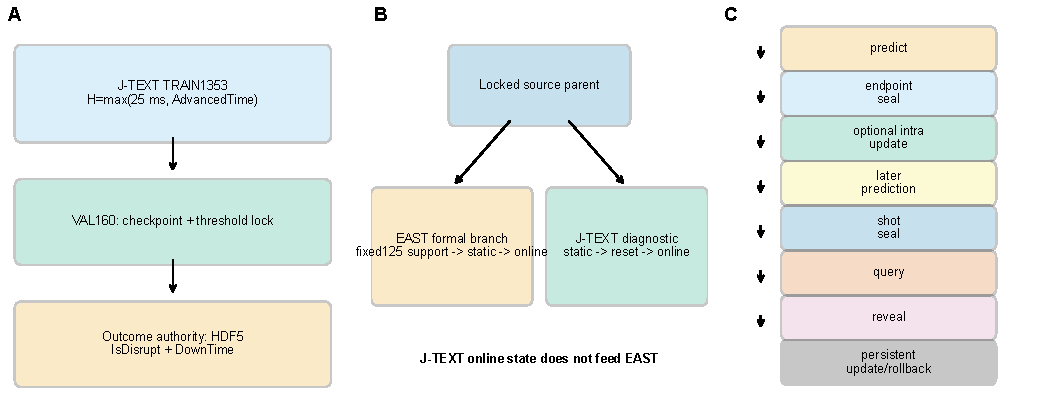
\includegraphics[width=\linewidth]{../figures_dynamic/F1_causal_data_role_pipeline.pdf}
\caption{数据角色、静态源父模型隔离和因果在线事件顺序。J-TEXT 在线状态不进入 EAST 迁移。}
\end{figure}

\section{数据角色、标签与时间口径}

\subsection{数据角色}

\begin{center}
\begin{tabular}{llll}
\toprule
装置与角色 & 炮数 & HDF5 构成 & 用途\\
\midrule
J-TEXT TRAIN1353 & 1353 & 188 破裂 & 源参数与 scaler\\
J-TEXT VAL160 & 160 & 80/80 & epoch 与阈值\\
J-TEXT TEST220 & 220 & 110/110 & 开发期比较及在线诊断\\
EAST support110 & 110 & 15/95 & 小样本迁移及阈值\\
EAST balanced360 & 360 & 180/180 & 静态与在线开发流\\
\bottomrule
\end{tabular}
\end{center}

support110 的 15 破裂/95 安全来自实际 HDF5；旧炮表标题中的 10/100 不作为标签权威。support110 与 balanced360 炮号互斥，但 balanced360 参与了方法开发，因此不是独立测试集。

\subsection{真值与正样本边界}

对炮 $s$，$d_s\in\{0,1\}$ 表示整炮结局，$t_s^{\mathrm{down}}$ 表示破裂时刻。二者分别只能来自 HDF5 \code{/meta/IsDisrupt} 和 \code{/meta/DownTime}。JSON AdvancedTime 仅是正样本时间窗的上界信息。

J-TEXT 的当前上界为
\begin{equation}
H_s^J=\max(25\ \mathrm{ms},A_s),
\label{eq:jtext-horizon}
\end{equation}
其中 $A_s$ 是 AdvancedTime；缺失时 $H_s^J=25$ ms。定义
\begin{equation}
\mathrm{TTD}_{s,t}=1000(t_s^{\mathrm{down}}-t)\ \mathrm{ms},
\end{equation}
则
\begin{equation}
y_{s,t}^{J}=\mathbf 1\{d_s=1,\ 0\leq\mathrm{TTD}_{s,t}\leq H_s^J\}.
\label{eq:jtext-label}
\end{equation}
EAST support110 保持固定 125 ms：
\begin{equation}
y_{s,t}^{E}=\mathbf 1\{d_s=1,\ 0\leq\mathrm{TTD}_{s,t}\leq125\ \mathrm{ms}\}.
\label{eq:east-label}
\end{equation}
因此当前标签臂是 \texttt{source\_dynamic\_\_east\_fixed}。它由开发期 $J=\mathrm{TPR}-\mathrm{FPR}$ 决定，不能被描述为预注册确认臂。

\subsection{报警与 operational 指标}

首次报警时间记为 $t_s^{\mathrm{alarm}}$，提前量为
\begin{equation}
\ell_s=1000(t_s^{\mathrm{down}}-t_s^{\mathrm{alarm}})\ \mathrm{ms}.
\end{equation}
J-TEXT operational TP 要求 $\ell_s>10$ ms；EAST 要求 $\ell_s\geq30$ ms。当前状态机不要求连续 10 点，任一因果端点满足冻结条件即可。早于破裂 3 s 以上的报警仍保留资格，但单独审计捷径。

\begin{equation}
\mathrm{TPR}=\frac{TP}{TP+FN},\qquad
\mathrm{FPR}=\frac{FP}{FP+TN},\qquad
J=\mathrm{TPR}-\mathrm{FPR}.
\label{eq:metrics}
\end{equation}
$TP,FP,TN,FN$ 分别是合格真阳性、假阳性、真阴性和操作假阴性。raw TPR 只说明发生过报警；提前量不足仍是 operational FN。本文主表不混用两种 TPR。

\section{共享表示与 J-TEXT 源模型}

\subsection{rebuilt17 与因果预处理}

共享主干使用 rebuilt17。J-TEXT 电流只执行一次 $I_p^A=1000I_p^{kA}$，并重构 $B_t/I_p$、$\Delta I_p(t)=I_p(t)-I_p(t-1)$ 和 $Z_{\mathrm{proxy}}=V_{\mathrm{loop}}/I_p$。TRAIN1353 拟合中位数 $m_c$ 与四分位距 $q_c$：
\begin{equation}
\tilde x_{t,c}=\operatorname{clip}
\left(\frac{x_{t,c}-m_c}{\max(q_c,10^{-6})},-10,10\right).
\label{eq:scaler}
\end{equation}
$x_{t,c}$ 是端点 $t$ 的通道 $c$，$\tilde x_{t,c}$ 是归一化值。EAST shared17 不重新拟合该 scaler。availability mask 区分缺测和物理零；短历史只在左侧补零，\texttt{valid\_lengths} 形成 patch mask，不读取未来端点。

\subsection{网络与源域损失}

输入是 $128\times17$ 因果窗；patch 宽 8、步长 8，共 16 个时间 token。模型含一个 CLS token、正弦位置编码、两层 4 头 Transformer，$d_{\mathrm{model}}=64$，FFN=256。风险头是 \texttt{64--64--GELU--Dropout(0.1)--1}。

\begin{equation}
\mathcal L_{\mathrm{src}}=-\frac1B\sum_{i=1}^{B}
[y_i\log\sigma(z_i)+(1-y_i)\log(1-\sigma(z_i))],
\label{eq:source-loss}
\end{equation}
其中 $B$ 是 batch 大小，$y_i$ 是窗口标签，$z_i$ 是风险 logit，$\sigma$ 为 sigmoid。AdamW 的学习率为 $3\times10^{-4}$，weight decay 为 $10^{-4}$，batch 128，梯度范数上限 1；最多 30 epoch、每 epoch 128 step、至少 12 epoch、patience 7。VAL160 先约束 timely TPR$\geq0.90$，再最小化 FPR；锁定 checkpoint 与阈值前 \texttt{test\_shards\_read=0}。

\section{J-TEXT 到 EAST 的小样本迁移}

\subsection{高层目标适配}

只加载同 seed 的静态 J-TEXT checkpoint。冻结 patch embedding、CLS 和第一层 Transformer；解冻最后一层及最终 LayerNorm；丢弃源风险头，初始化独立 EAST 风险头。support110 上的目标为
\begin{equation}
\mathcal L_{\mathrm{adapt}}=
\operatorname{BCEWithLogits}(z_{s,t}^{E},y_{s,t}^{E}).
\end{equation}
训练 12 epoch，每 epoch 32 batch，batch 128，AdamW 学习率 $10^{-4}$。support110 还用于选择满足 timely TPR$\geq0.80$ 时 FPR 最低的目标阈值，故不存在独立目标验证。

\subsection{共享动态残差}

\begin{equation}
\delta_t^{\mathrm{shared}}=
g_t\tanh f_{\mathrm{shared}}(h_t,q_t,a_t,z_t^0),
\qquad|\delta_t^{\mathrm{shared}}|\leq1.
\label{eq:shared}
\end{equation}
$h_t$ 是隐藏状态，$q_t$ 是共享物理向量，$a_t$ 是可用掩码，$z_t^0$ 是基础 logit，$g_t$ 是物理可用门。其支持集损失为
\begin{equation}
\mathcal L_{\mathrm{DHA}}=\mathcal L_{\mathrm{BCE}}
+0.20\mathcal L_{\mathrm{next}}
+1.00\mathcal L_{\mathrm{anchor}}
+0.05\,\mathbb E[(\delta_t^{\mathrm{shared}})^2].
\label{eq:dha}
\end{equation}
$\mathcal L_{\mathrm{next}}$ 重建下一因果状态，$\mathcal L_{\mathrm{anchor}}$ 保护已判对的支持窗口。

\subsection{EAST-private raw8}

不强制对齐的 8 个 EAST 通道各提取 6 个因果摘要，形成 48 维 $r_t$：
\begin{equation}
\delta_t^{\mathrm{private}}=
0.5\tanh f_{\mathrm{private}}(r_t,z_t^{\mathrm{shared}}),
\qquad|\delta_t^{\mathrm{private}}|\leq0.5,
\end{equation}
\begin{equation}
z_t^E=z_t^0+\delta_t^{\mathrm{shared}}+\delta_t^{\mathrm{private}}.
\label{eq:target-logit}
\end{equation}
这意味着 23 维并未简单丢弃：shared17 负责跨装置可比较表示，raw8 只在 EAST 小支路中补充目标表象。

\section{EAST 在线主动适配}

每炮顺序是：预测、端点封存、可选炮内 fast 更新、整炮封存、查询、仅选中炮揭示、persistent 更新或回滚。当前炮结局和未来端点不可进入当前预测。

每炮开始从 persistent 深复制 fast；炮内无标签梯度只改变 fast，炮后丢弃，persistent 哈希必须不变。EAST 查询结合报警边界不确定性和模型--物理矛盾，并使用滚动 token 预算。配置为：20 炮名义配额 4、历史 80、分位数 0.8、不确定性权重 0.65、初始 cutoff 0.35、token capacity 12；三 seeds 实际查询 63/63/62 炮。

炮间仅在选中炮封存后读取标签。更新含部署边界监督、replay、物理、下一状态与 guard。更新前保存模型和优化器；非有限损失、梯度、参数、优化器状态或 guard 失败均回滚。新 persistent 只影响后续炮。

\section{J-TEXT TEST220 在线诊断支路}

\subsection{有界残差与炮内损失}

在线模块只有 2241 个可训练参数，源 encoder/head 冻结：
\begin{equation}
z_t=z_t^0+\Delta z_t,\qquad
\Delta z_t=0.5\tanh f_{\mathrm{res}}(x_t,a_t,\sigma(z_t^0)).
\end{equation}
零初始化保证初始输出等于静态父模型。实际炮内损失为
\begin{equation}
\mathcal L_{\mathrm{intra}}=
1.0\mathcal L_{\mathrm{next}}+
0.5\mathcal L_{\mathrm{teacher}}+
0.25\mathcal L_{\mathrm{anchor}}+
0.0\mathcal L_{\mathrm{physics}}.
\label{eq:j-intra}
\end{equation}
最后一项权重为 0，不能写成生效贡献。

\subsection{查询价值}

风险概率序列为 $p_1,\ldots,p_T$：
\begin{equation}
U=\frac1T\sum_{t=1}^{T}(1-|2p_t-1|),
\end{equation}
\begin{equation}
\Delta_x=\frac{\operatorname{mean}|x_T-x_1|}
{1+\operatorname{mean}|x_T-x_1|},\qquad
C=\operatorname{clip}(\lvert |p_T-p_1|-\Delta_x\rvert,0,1).
\end{equation}
$U$ 是不确定性，$C$ 是风险变化与特征变化的矛盾度。炮表型
$\phi=[\operatorname{mean}(p),\max(p),p_T-p_1,\Delta_x]$。只在过去已查询并揭示的表型库 $\mathcal M$ 中计算
\begin{equation}
N=\operatorname{clip}
\left(\min_{\psi\in\mathcal M}
\sqrt{\operatorname{mean}(\phi-\psi)^2},0,1\right),
\end{equation}
空库时 $N=0$。最终
\begin{equation}
V=wU+(1-w)C+\eta N,\qquad w=0.65,\quad\eta=0.10.
\label{eq:query}
\end{equation}
20\% 预算按连续 20 炮块恰好查询 4 炮，共 44 炮。先选 $V\geq0.5$ 的炮，块末用 causal forced-fill 补足预算。10\%/30\% 对应 22/66 炮。

\subsection{炮间损失与事务保护}

每次查询取当前 8 窗、replay 8 窗、guard 8 窗，执行 2 个 optimizer steps：
\begin{equation}
\mathcal L_{\mathrm{inter}}=
1.0\mathcal L_{\mathrm{sup}}+
0.5\mathcal L_{\mathrm{replay}}+
0.25\mathcal L_{\mathrm{anchor}}+
0.0\mathcal L_{\mathrm{physics}}.
\label{eq:j-inter}
\end{equation}
三个 seeds 均查询 44 炮、尝试 88 步、无回滚；active 与 random 的窗口和报告 FLOPs 匹配。

\section{结果与裁决}

\begin{center}
\small
\begin{tabular}{rrrrrrrr}
\toprule
seed & J-T TPR & J-T FPR & J-T AUC & E-S TPR & E-S FPR & E-O TPR & E-O FPR\\
\midrule
131 & .900000 & .154545 & .978926 & .866667 & .138889 & .861111 & .138889\\
133 & .836364 & .100000 & .961736 & .766667 & .122222 & .766667 & .116667\\
137 & .863636 & .136364 & .963058 & .838889 & .166667 & .844444 & .172222\\
均值 & \textbf{.866667} & \textbf{.130303} & \textbf{.967906} &
\textbf{.824074} & \textbf{.142593} & \textbf{.824074} & \textbf{.142593}\\
\bottomrule
\end{tabular}
\end{center}

EAST online 相对 static 的 $\Delta J$ 按 seed 为 $-0.005556、+0.005556、0$。三 seed 变化相互抵消，不能表述为稳定在线增益。该结果来自恢复后的历史炮优先 support110 采样器和未经删改的原 v3c 在线配置。

J-TEXT static、EAST static、EAST online 的 $J$ 分别为 0.736364、0.681481、0.681481。EAST 在线三 seed 平均 $\Delta J=0$。seed133 TPR 未达到 0.80，故 \texttt{T0\_ADMITTED=false}。

J-TEXT 20\% full-active 相对 static 的 $\Delta J$ 为 0、$-0.009091$、0，故 \texttt{ONLINE\_SUPPORTED=false}。seed131 的 10\%/20\%/30\% 预算均不改变炮级指标。active 与 equal-compute random 的 44 炮集合只重合 4 炮，却都只覆盖 6 个静态错误型炮。44 个前缀标签直接训练的后缀对照从 $J=0.763025$ 降到 0.751261；这反驳“标签数相同就必然提升”，但不证明主动策略优越。

\begin{figure}[htbp]
\centering
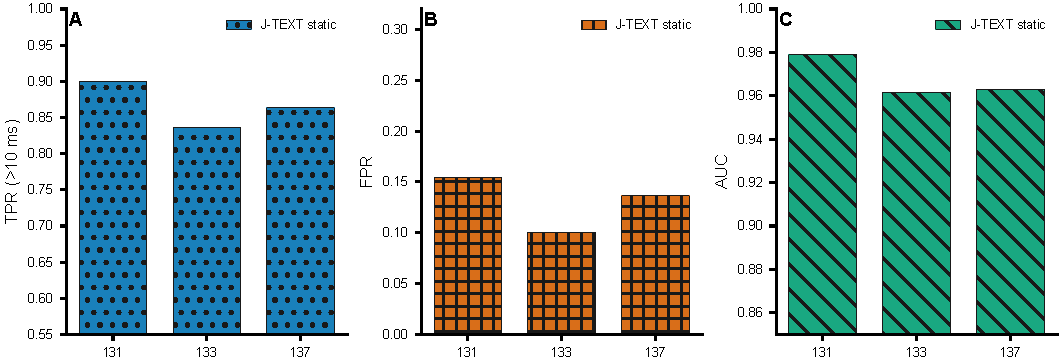
\includegraphics[width=\linewidth]{../figures_dynamic/F2_jtext_source_three_seed.pdf}
\caption{J-TEXT TEST220 三随机种子源模型表现。每根柱对应一个独立训练 seed，不把 220 炮伪作独立重复。}
\end{figure}

\begin{figure}[htbp]
\centering
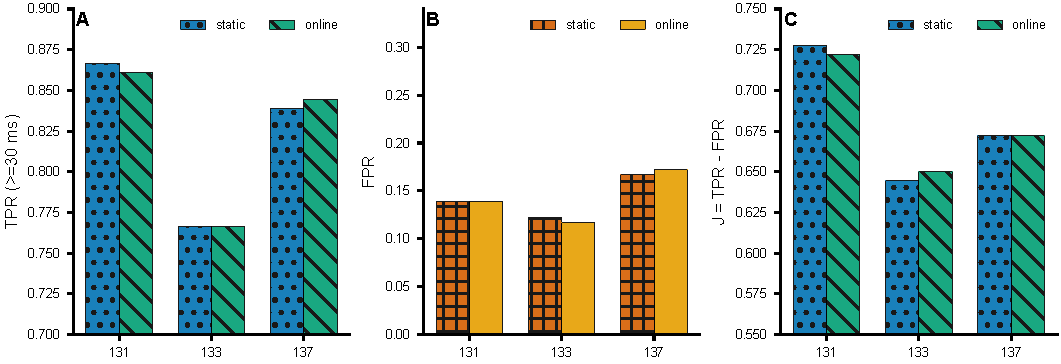
\includegraphics[width=\linewidth]{../figures_dynamic/F3_east_static_online_three_seed.pdf}
\caption{EAST balanced360 上同父模型静态与在线对照。在线增益主要来自及时 TPR，FPR 未下降。}
\end{figure}

\begin{figure}[htbp]
\centering
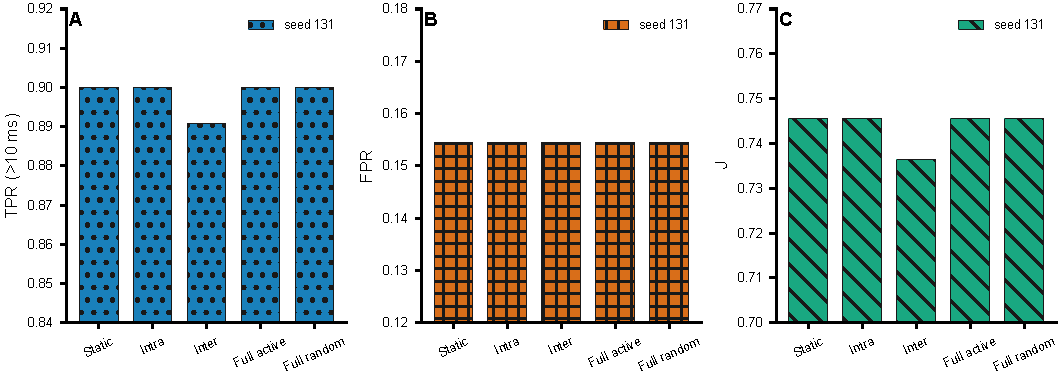
\includegraphics[width=\linewidth]{../figures_dynamic/F4_jtext_online_ablation.pdf}
\caption{J-TEXT seed131 的炮内、炮间、完整主动与等计算随机查询消融。}
\end{figure}

\begin{figure}[htbp]
\centering
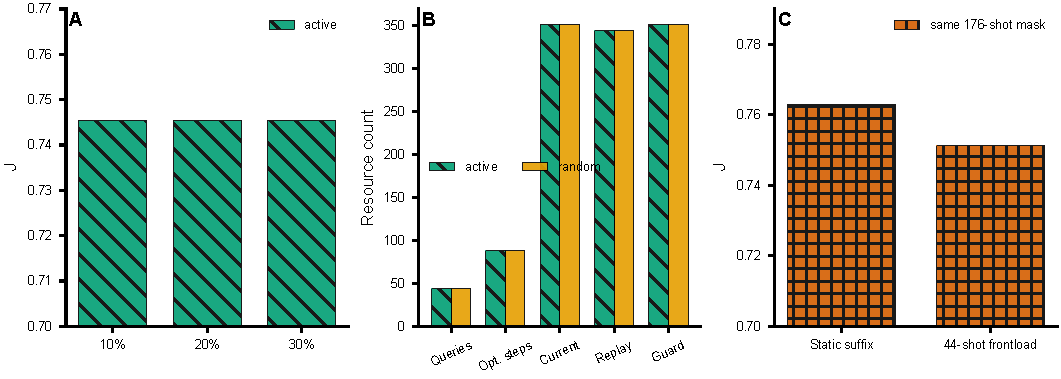
\includegraphics[width=\linewidth]{../figures_dynamic/F5_budget_falsification_controls.pdf}
\caption{查询预算、等资源随机对照与 44 炮前置直接训练的共同后缀比较。}
\end{figure}

\okbox{\textbf{工程结论。} 静态源、目标小样本迁移、静态封存、顺序在线、查询揭示和事务更新已形成一条可执行链路。}
\riskbox{\textbf{科学结论。} 当前结果未达到 EAST admission，也未支持 J-TEXT 在线主动增益。balanced360 和 TEST220 上的结果都只能作为开发证据。}

\section{符号与缩写}

\begin{longtable}{p{0.23\linewidth}p{0.68\linewidth}}
\toprule
符号或缩写 & 定义\\
\midrule
$s,t$ & 炮编号与炮内因果端点\\
$d_s,t_s^{\mathrm{down}}$ & HDF5 结局与破裂时刻\\
$A_s,H_s^J$ & AdvancedTime 与 J-TEXT 正样本上界\\
TTD & time to disruption，距离破裂的剩余时间\\
$x_t,a_t$ & rebuilt17 特征与可用掩码\\
$h_t,q_t,r_t$ & 隐状态、共享物理向量、EAST raw8 摘要\\
$z,p$ & 风险 logit 与 sigmoid 风险概率\\
$\delta^{\mathrm{shared}},\delta^{\mathrm{private}}$ & 共享与目标私有 logit 残差\\
$U,C,N,V$ & 不确定性、矛盾度、新颖度、查询价值\\
$w,\eta$ & 查询混合权重与新颖度系数\\
fast/persistent & 炮内临时模型与跨炮慢状态\\
TP/FP/TN/FN & 真阳性、假阳性、真阴性、操作假阴性\\
TPR/FPR/AUC/$J$ & 真阳性率、假阳性率、ROC AUC、TPR$-$FPR\\
SHA-256 & 绑定代码、数据、模型和证据字节的哈希\\
\bottomrule
\end{longtable}

\section{公式与代码映射}

\begin{longtable}{p{0.34\linewidth}p{0.57\linewidth}}
\toprule
公式或过程 & 代码入口\\
\midrule
式(\ref{eq:jtext-horizon})--(\ref{eq:east-label}) & \code{advanced_time_labels.py}; \code{train_jtext_source_transformer.py}\\
式(\ref{eq:scaler})与 rebuilt17 & \code{rebuilt_harness.py}\\
式(\ref{eq:source-loss})与 Transformer & \code{grid_search.py::Enc/Head}; \code{train_jtext_source_transformer.py}\\
高层 EAST 适配 & \code{grid_search.py::train_adapt}; \code{run_selected_full_mainline.py}\\
式(\ref{eq:shared})--(\ref{eq:dha}) & \code{dynamic_hazard_adapter.py}; \code{run_dynamic_hazard_adapter.py}\\
式(\ref{eq:target-logit}) & \code{east_private23_sidecar.py}; \code{east_private_continual.py}\\
EAST 顺序在线 & \code{run_unified_online_active.py}; \code{unified_online_value.py}\\
式(\ref{eq:j-intra})、(\ref{eq:j-inter}) & \code{jtext_online_adapter.py}\\
式(\ref{eq:query}) & \code{run_jtext_online_active.py::JTextQueryValue}\\
最终证据核验 & \code{paper_grade_package/scripts/build_dynamic_mainline_evidence.py} 与最终装配脚本\\
报告合同与编译 & \code{paper_grade_package/scripts/build_dynamic_report.py}\\
\bottomrule
\end{longtable}

\section{复现命令}

\begin{verbatim}
cd /path/to/tokamak-final
export FUSION_DATA_ROOT=/path/to/data
PY=${CONDA_PREFIX}/bin/python

$PY -c 'import torch,h5py; print(torch.cuda.is_available())'

for seed in 131 133 137; do
  $PY experiments/transfer_methods_2026/run_selected_full_mainline.py \
    --seed "$seed" --stage all \
    --data-root "$FUSION_DATA_ROOT" \
    --output "/ext4/runs/selected_full_mainline/seed${seed}"
done

$PY experiments/transfer_methods_2026/paper_grade_package/scripts/\
build_dynamic_report.py --check-only
$PY experiments/transfer_methods_2026/paper_grade_package/scripts/\
build_dynamic_report.py
$PY -m pytest -q tests/experiments/test_dynamic_mainline_report.py
\end{verbatim}

跨机复现还必须保存代码 SHA、配置 SHA、HDF5 内容清单、炮表 SHA、checkpoint SHA、阈值回执、逐炮预测和查询/更新回执。单独复现汇总表不等于复现完整主线。

\section{当前结论}

工程链路已经打通并可审计，逐炮证据重算与哈希核验也已完成；EAST admission 与 J-TEXT \texttt{ONLINE\_SUPPORTED} 均未通过。下一步是在新未来流上预注册确认。不能继续在 balanced360 或 TEST220 上追逐参数后把结果升级为确认性结论。

\end{document}
